\documentclass{article}
\usepackage{graphicx}
\usepackage{amsmath}
\graphicspath{ {./images/} }
\title{Winning at Monopoly \\ \large The mathematics behind the game of Monopoly }
\author{Lars Kwant}

\begin{document}

\maketitle

\tableofcontents

\newpage

\section{Introduction to the game}
\subsection{Goal of the game}
Monopoly is a game played by 2 to 6 individuals. The goal of the game is to become the player that does not go bankrupt. The goal of each individual is therefore to make as much money as possible in order to make each opponent go bankrupt. The player does this by buying property and issuing rent on opponents if they land on one of these properties.\\

\subsection{The board}
The board is seperated into 40 squares. Each square has its own unique action attached to it. 
\begin{figure}[h]
\centering
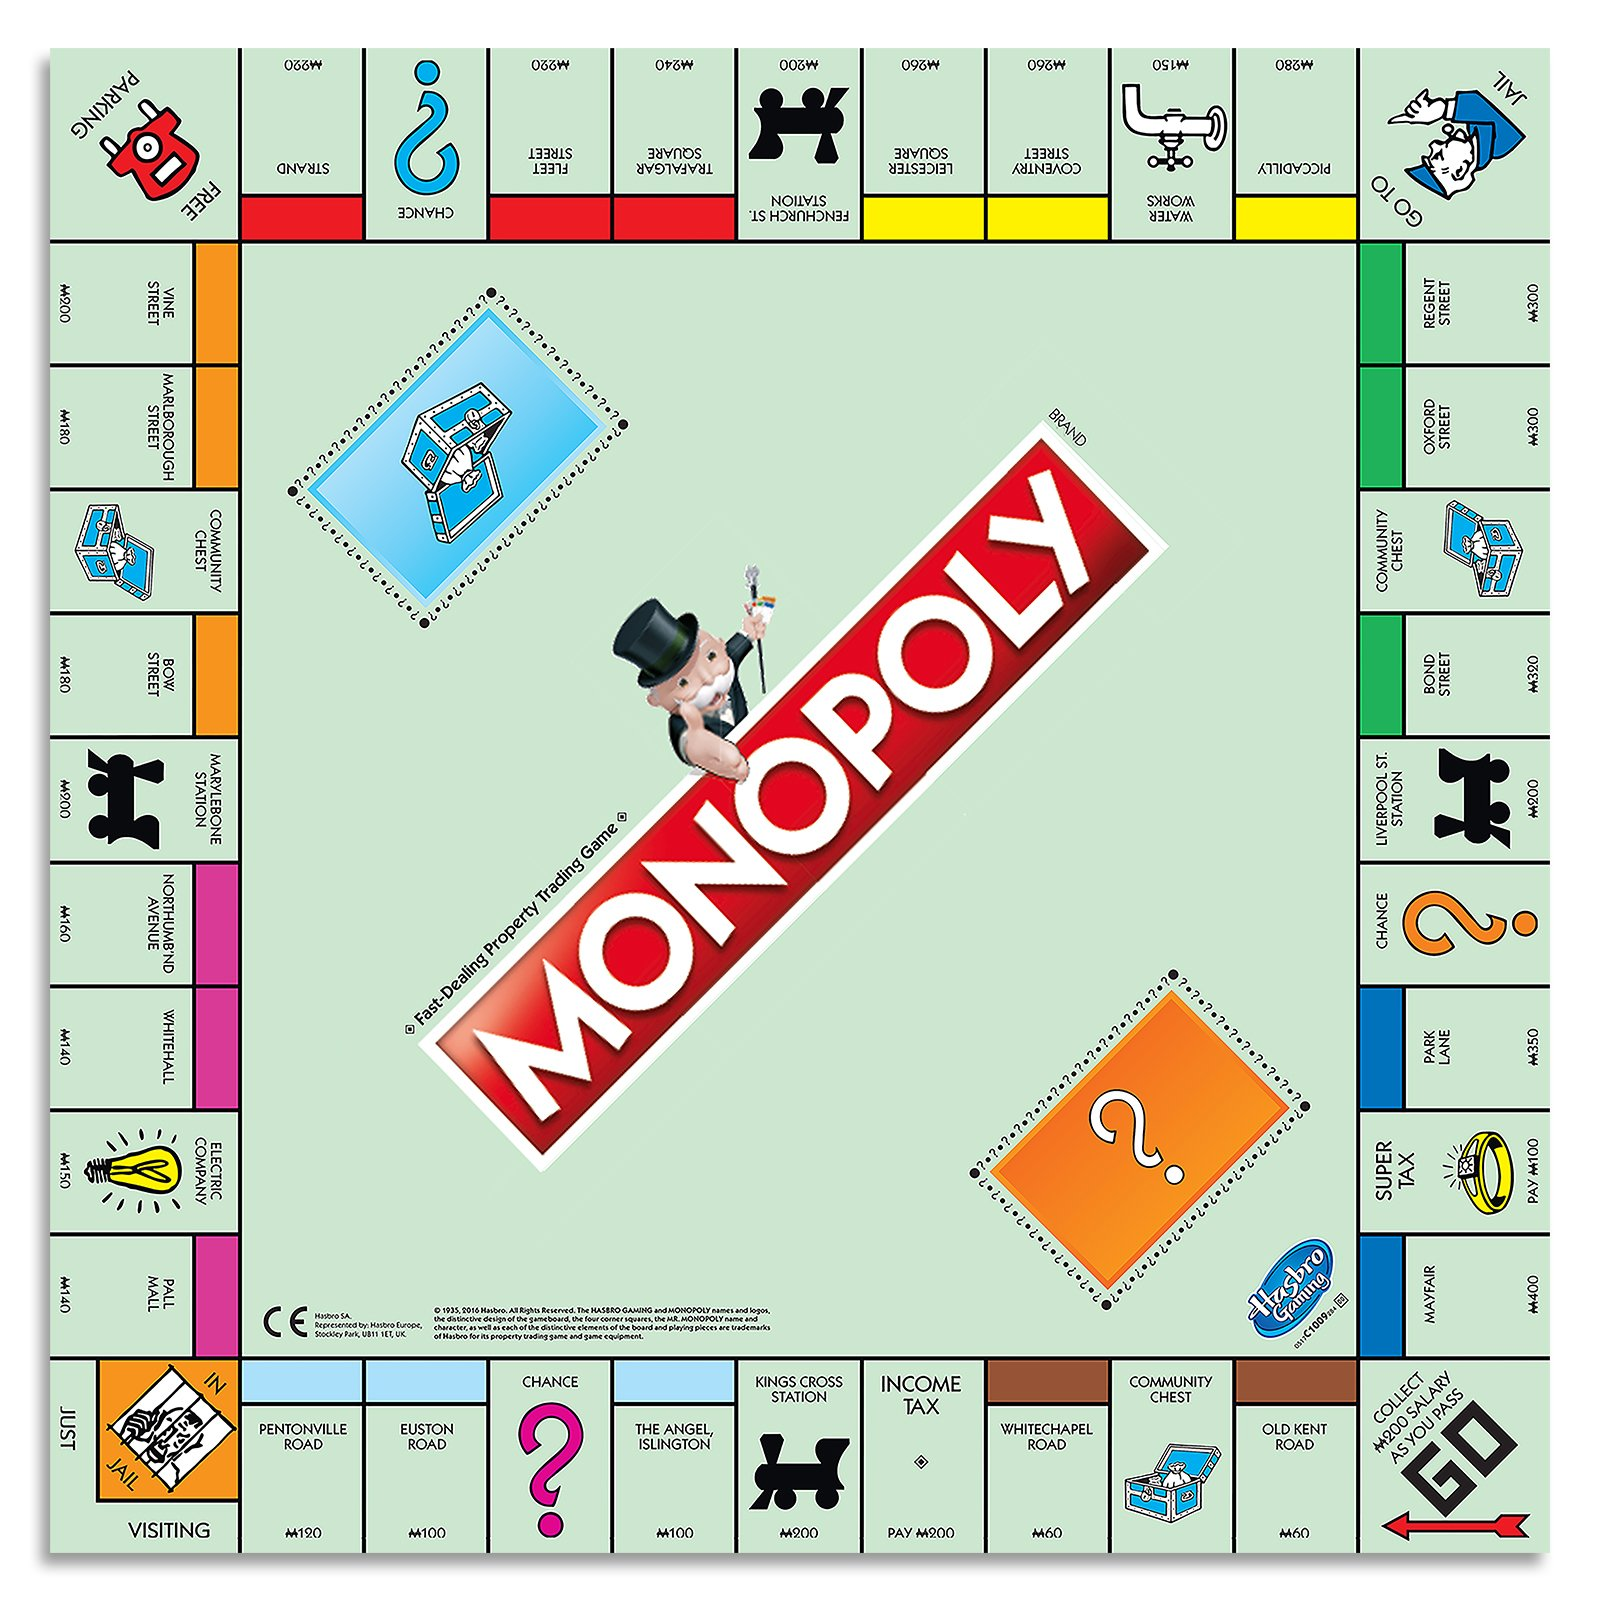
\includegraphics[width = 0.7\textwidth]{images/board.jpg}
\caption{The classic Monopoly board \cite{mon_board_image}}
\end{figure}
\textit{To be expanded...}

\section{Throwing the die}
Monopoly is generally played with 2 dice. For us to figure out what is the best way to play Monopoly it might come in handy to find out what are the exact odds of ending on a certain square. For this we first need to go over some basic probability theory. Assuming that all dice that come delivered with the game box are fair, we can assume that the result of a single die throw is discrete uniformly distributed on the set $\{1,2,3,4,5,6\}$. Let $X$ be the random variable corresponding to the total throw. We can then construct its PMF:
$$P(X = x) = P(X_1 + X_2 = x)$$
We can construct a simple table to find all possible throws, and then calculate the probabilities of throwing that number.


\begin{table}[h]
\centering
\begin{tabular}{|c|c|c|c|c|c|c|}
 Die rolls& 1 & 2 & 3 & 4 & 5 & 6 \\
 \hline
 1& 2 & 3 & 4 & 5 & 6 & 7\\
 \hline
 2& 3 & 4 & 5 & 6 & 7 & 8\\
 \hline
 3& 4 & 5 & 6 & 7 & 8 & 9\\
 \hline
 4& 5 & 6 & 7 & 8 & 9 & 10\\
 \hline
 5& 6 & 7 & 8 & 9 & 10 & 11\\
 \hline
 6& 7 & 8 & 9 & 10 & 11 & 12\\
\end{tabular}
\caption{All possible die throws}
\end{table}

Counting all possibilities we obtain the following PMF for $X$ (The total number of steps):

\begin{figure}[h]
\centering
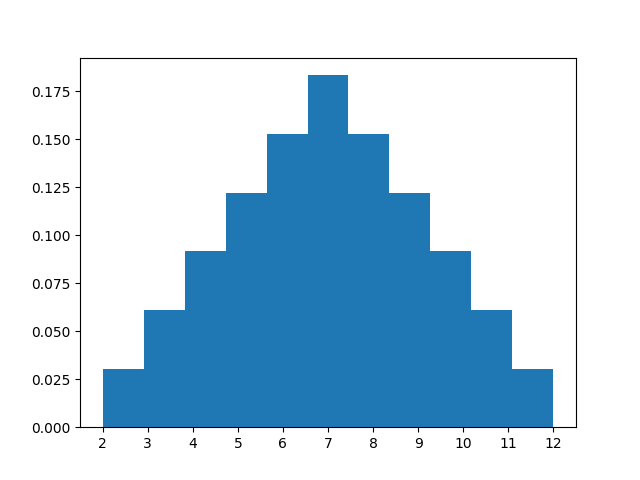
\includegraphics[width = 0.7\textwidth]{die_roll_histogram.png}
\caption{Probability mass of each possible die throw}
\end{figure}

It's clear to see that a player is most likely to throw a $7$. The exact probability is:
$$P(X = 7) = \frac{1}{6}$$

If we for example consider the first turn we can create a simple heat map of the probability of ending on any square.


\begin{figure}[h]
\centering
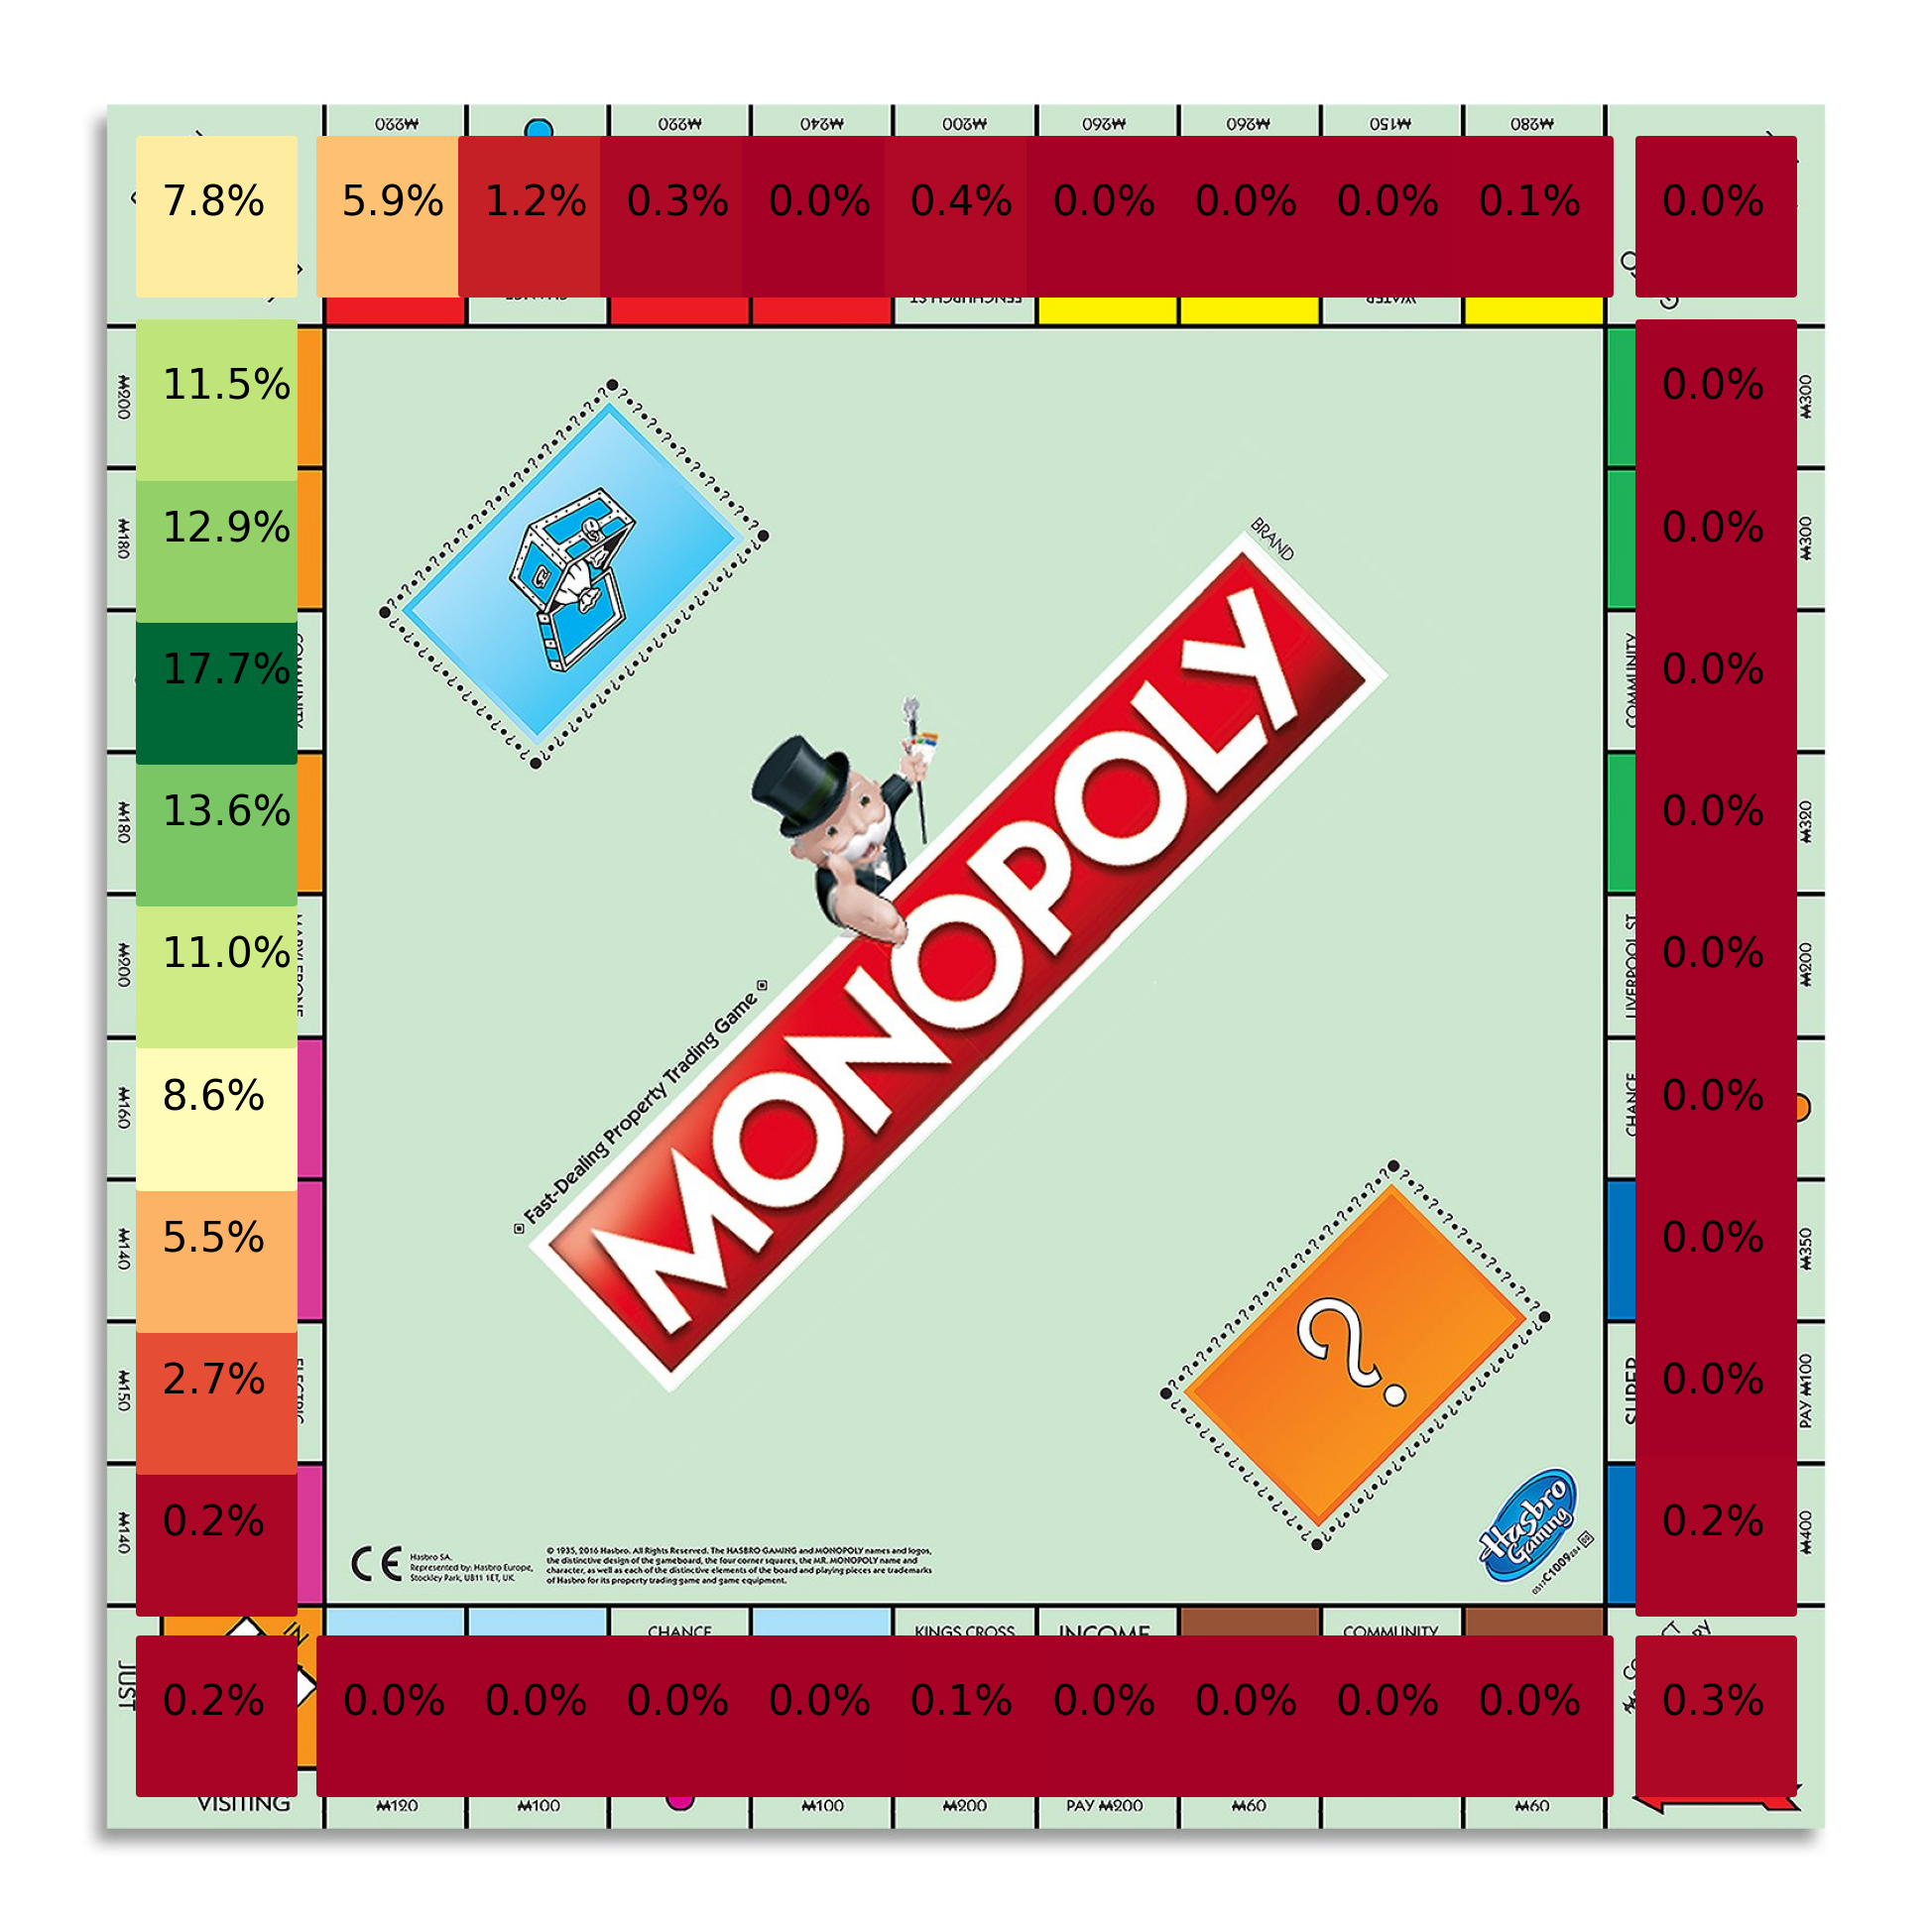
\includegraphics[width = 0.7\textwidth]{firstThrow.png}
\caption{Probability of ending up on a certain spot on the first throw}
\end{figure}

Note that some squares also have small probability mass even though they are not reachable from start directly. This is because the chance card allows the player to move to different squares. The player has a $1.1\%$ chance of traveling to start in one throw.

\begin{thebibliography}{9}
\bibitem{mon_board_image} This is some information about the source
\end{thebibliography}

\end{document}